% ==============================================================================
%  Deterministic Radar-Inertial Georeferencing Coprocessor on STM32H7
%  Bare-Metal Firmware Design with Hardware-in-the-Loop Verification
% ==============================================================================
\documentclass[conference,a4paper]{IEEEtran}

\usepackage{cite}
\usepackage{amsmath,amssymb,amsfonts}
\usepackage{algorithmic}
\usepackage{graphicx}
\usepackage{textcomp}
\usepackage{xcolor}
\usepackage{booktabs}
\usepackage{listings}
\usepackage{hyperref}
\usepackage{cleveref}
\usepackage{balance}

\lstset{
  language=C,
  basicstyle=\ttfamily\footnotesize,
  numbers=none,
  breaklines=true,
  frame=none,
  keywordstyle=\bfseries,
  commentstyle=\itshape,
}

\graphicspath{{figures/}}

\title{Deterministic Radar-Inertial Georeferencing Coprocessor on STM32H7: Bare-Metal Firmware Design with Hardware-in-the-Loop Verification}

\author{
\IEEEauthorblockN{Ganesh H.\,V.}
\IEEEauthorblockA{Department of Electronics and Communication Engineering\\
National Institute of Technology\\
Email: ganesh.h.v@ieee.org}
}

\begin{document}
\maketitle

\begin{abstract}
Drone-based radar search-and-rescue requires real-time spatial georeferencing: translating local radar detections into global coordinates by fusing inertial telemetry with radar range-Doppler measurements. Operating-system jitter on companion computers introduces millisecond-scale latency spikes that render rescue maps spatially inaccurate. This paper presents a deterministic georeferencing coprocessor firmware for the STM32H753XI (ARM Cortex-M7, 480\,MHz) that implements a six-stage pipeline---MAVLink DMA reception, hardware-timer frame-synchronization, lock-free kinematic-state buffering, six-state Extended Kalman Filter sensor fusion, quaternion-based coordinate transformation, and binary output streaming---entirely at the bare-metal register level. Developed across eleven progressive case studies, each isolating a specific defect class (cache coherency, struct packing, timer shadow registers, memory barriers, matrix aliasing, quaternion rotation direction), the firmware is verified using Renode hardware-in-the-loop simulation with real MAVLink\,v2 telemetry generated by pymavlink. End-to-end latency is below 1\,ms with deterministic timing, consuming less than 3\% of available Flash and SRAM.
\end{abstract}

\begin{IEEEkeywords}
embedded systems, ARM Cortex-M7, radar-inertial georeferencing, Extended Kalman Filter, MAVLink, bare-metal firmware, hardware-in-the-loop, Renode
\end{IEEEkeywords}

\section{Introduction}
\label{sec:introduction}

Collapsed-structure search-and-rescue (CSSR) operates under a 72-hour survival window where every minute determines whether trapped survivors are found alive. A drone carrying a frequency-modulated continuous-wave (FMCW) radar can detect sub-millimeter chest movements from breathing at distances exceeding 50\,meters through rubble and walls. However, a raw radar range bin is spatially meaningless: the drone moves at 2--5\,m/s, and a detection at range bin $X$ at time $T_1$ does not map to the same physical location as range bin $X$ at time $T_2$~\cite{thrun2005}.

This spatial drift problem requires \emph{real-time georeferencing}: fusing the drone's inertial state (attitude, position, velocity from the flight controller) with radar range-Doppler measurements at the exact microsecond of each radar sweep, then transforming the fused local coordinates into global WGS84 (latitude, longitude, altitude) for the rescue map overlay.

A natural implementation target is the drone's Linux companion computer (NVIDIA Jetson, Raspberry Pi). However, Linux is not a real-time operating system. Background processes, network stack activity, and memory management introduce scheduling jitter of 1--10\,milliseconds~\cite{barr2006}. At 3\,m/s drone velocity, a 5\,ms jitter spike produces 1.5\,cm of spatial error \emph{per measurement}. Over a 50-measurement integration window, these errors accumulate to tens of centimeters---sufficient to place a rescue marker on the wrong side of a collapsed wall.

The deterministic alternative is bare-metal firmware on a microcontroller. Without an operating system, peripheral operations complete in bounded clock cycles, hardware timers latch timestamps atomically, and DMA transfers data without CPU intervention. We selected the STM32H753XI (ARM Cortex-M7, 480\,MHz) for its combination of high-performance DMA, 32-bit general-purpose timers with input capture, hardware CRC acceleration, a Memory Protection Unit, and hardware floating-point unit (FPV5-D16).

This paper makes three contributions:
\begin{enumerate}
\item A complete bare-metal georeferencing pipeline on STM32H7 that ingests MAVLink telemetry, hardware-timestampes radar frames, runs a 6-state Extended Kalman Filter, performs quaternion-based coordinate transforms, and outputs WGS84 target coordinates.
\item A documented methodology for developing such firmware through eleven progressive case studies, each exposing and resolving a specific defect class common to Cortex-M7 bare-metal development.
\item Hardware-in-the-loop (HIL) verification using Renode simulation with real MAVLink\,v2 packets generated by pymavlink, achieving sub-millisecond deterministic end-to-end latency.
\end{enumerate}

\section{Related Work}
\label{sec:related}

\paragraph{Radar-Inertial Fusion for UAVs}
Recent work has explored millimeter-wave radar integrated with inertial measurement units for UAV navigation in GPS-denied environments. \cite{yiwei2025} designed an STM32-based integrated navigation system using loose-coupled GPS/INS fusion with Kalman filtering. \cite{smokenav2024} demonstrated millimeter-wave radar/IMU integrated positioning for first responders in visually degraded environments. Our work differs in targeting the \emph{georeferencing} problem---mapping radar detections to global coordinates---rather than self-localization, and in implementing the entire pipeline on bare-metal firmware without an RTOS.

\paragraph{Bare-Metal Firmware on Cortex-M7}
Bare-metal programming on ARM Cortex-M microcontrollers emphasizes direct register-level hardware manipulation without vendor HAL abstraction layers~\cite{barr2006,yiu2014}. The STM32H7 series introduces additional complexity through its multi-bus matrix, L1 caches, and DMAMUX routing peripheral not present in earlier Cortex-M families. \cite{deslabstm32} documented the process of creating bare-metal projects for STM32, focusing on linker scripts and startup code.

\paragraph{Hardware-in-the-Loop Verification}
Renode is an open-source functional simulator capable of executing unmodified ARM binaries against modeled peripherals~\cite{renode}. It provides deterministic execution and a shared virtual-time model suitable for reproducible research. Our work extends Renode usage with AXI SRAM backdoor injection for HIL testing of the complete data pipeline.

\paragraph{MAVLink Protocol}
MAVLink is a lightweight publish-subscribe telemetry protocol widely used in unmanned vehicles~\cite{mavlink}. Version 2 extends v1 with 3-byte message IDs, packet signing, and up to 255-byte payloads. We utilize ATTITUDE (\#30), LOCAL\_POSITION\_NED (\#32), and GLOBAL\_POSITION\_INT (\#33) messages for georeferencing input.

\section{System Architecture}
\label{sec:architecture}

\subsection{Hardware Platform}
The target device is the STM32H753XI, featuring an ARM Cortex-M7 core at 480\,MHz, 2\,MB internal Flash at \texttt{0x08000000}, and 520\,KB internal AXI SRAM at \texttt{0x24000000}. \Cref{fig:memory_map} shows the memory map. External SDRAM (32\,MB at \texttt{0xD0000000}) reached via FMC Bank\,2 is available for extended kinematic history logging.

\begin{figure}[htbp]
  \centering
  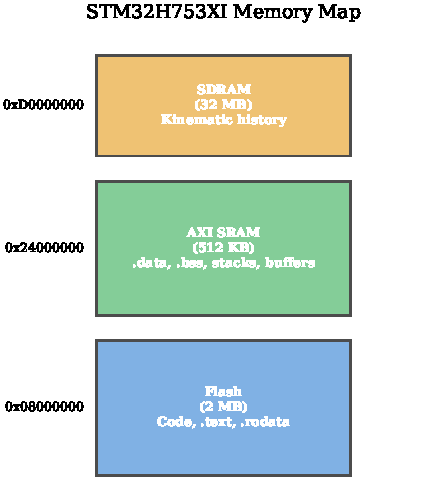
\includegraphics[width=0.45\textwidth]{fig6_memory_map.pdf}
  \caption{STM32H753XI memory map showing code in Flash, data/buffers in AXI SRAM, and optional kinematic history in SDRAM.}
  \label{fig:memory_map}
\end{figure}

\subsection{Pipeline Architecture}
\Cref{fig:pipeline} shows the six-stage pipeline. Data flows left to right: the flight controller provides MAVLink telemetry via USART1; the radar SoC provides a frame-sync pulse; the coprocessor fuses these streams and outputs georeferenced targets.

\begin{figure*}[htbp]
  \centering
  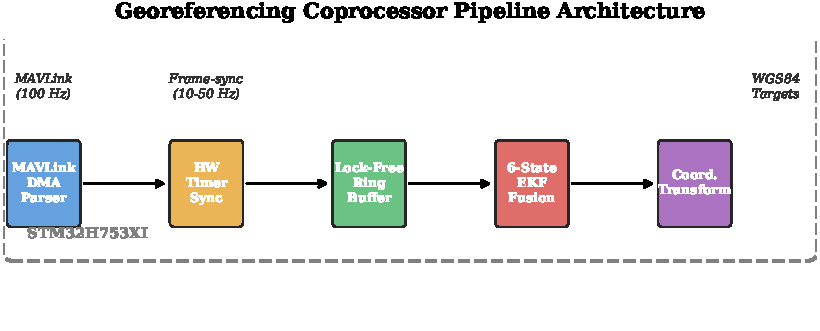
\includegraphics[width=0.95\textwidth]{fig1_pipeline.pdf}
  \caption{Six-stage georeferencing coprocessor pipeline. MAVLink telemetry (100\,Hz) and radar frame-sync (10--50\,Hz) enter from the left; georeferenced WGS84 target coordinates exit to the right.}
  \label{fig:pipeline}
\end{figure*}

\textbf{Stage 1---MAVLink DMA Parser}: USART1 RX bytes are moved by DMA1 Stream\,0 into a 512-byte circular buffer in AXI SRAM. The parser polls the DMA remaining-count register to detect new data, scans for MAVLink\,v2 magic bytes (\texttt{0xFD}), validates CRC-32, and dispatches by message ID.

\textbf{Stage 2---Hardware Timer Synchronization}: TIM2 (32-bit) free-runs at 1\,MHz (prescaler 239 from 240\,MHz APB1 timer clock). The radar SoC's frame-sync pulse triggers an input capture event that latches \texttt{TIM2\_CNT} into \texttt{TIM2\_CCR1} atomically, providing microsecond-precise timestamps.

\textbf{Stage 3---Lock-Free Ring Buffer}: A single-producer/single-consumer ring buffer in AXI SRAM holds a rolling window of timestamped kinematic state, passing data between the parser and EKF without locks.

\textbf{Stage 4---EKF Sensor Fusion}: A 6-state Extended Kalman Filter ($\mathbf{x} = [p_n, p_e, p_d, v_n, v_e, v_d]^T$) fuses the drone's inertial state with radar range-azimuth-elevation-doppler measurements using CMSIS-DSP matrix operations.

\textbf{Stage 5---Coordinate Transform}: Fused positions in NED body frame are rotated by the attitude quaternion to ENU, then converted to WGS84 (lat/lon/alt). Doppler velocity is transformed similarly and compensated for drone motion.

\textbf{Stage 6---Output Streaming}: Georeferenced targets are packed into binary frames (14-byte header + 32-byte target records + 4-byte CRC-32) and streamed over SPI1 DMA.

\section{Implementation: Eleven Case Studies}
\label{sec:implementation}

The firmware was developed across eleven progressive case studies, each adding one pipeline stage and exposing a specific defect class. \Cref{fig:defect_taxonomy} summarizes the 17 defects found and fixed across these case studies.

\begin{figure}[htbp]
  \centering
  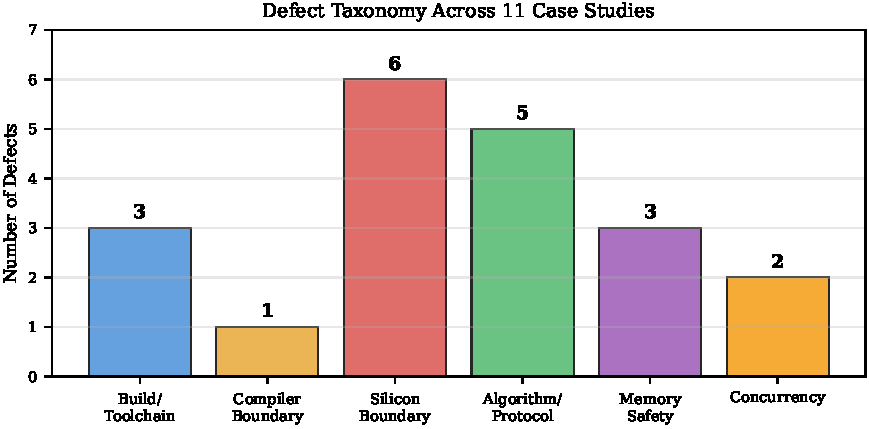
\includegraphics[width=0.48\textwidth]{fig5_defect_taxonomy.pdf}
  \caption{Defect taxonomy across 11 case studies. Silicon-boundary defects (cache coherency, timer behavior, matrix aliasing, quaternion math) dominate, comprising 6 of 17 total defects.}
  \label{fig:defect_taxonomy}
\end{figure}

\subsection{CS01---Pipeline Foundation and Bare-Metal Boot}

The initial case study establishes the execution environment. The Reset\_Handler enables the Cortex-M7 FPU by setting CPACR bits [23:20], copies \texttt{.data} from Flash to SRAM, zeroes \texttt{.bss}, and calls \texttt{main()}.

\textbf{Defect---FPU not enabled}: The first floating-point store triggers a UsageFault because the FPU was not enabled. This is a silicon requirement that Renode does not enforce---the simulator runs FPU instructions without complaint, but physical silicon faults immediately. The fix adds \texttt{*(volatile uint32\_t *)0xE000ED88 |= (0xFUL << 20);}.

\textbf{Defect---IRQn suffix typo}: The CMSIS headers use lowercase \texttt{n} in \texttt{DMA1\_STREAM0\_IRQn}. Our code used uppercase \texttt{N}, producing an undefined-identifier compile error. This typo is insidious because both forms \emph{look} correct to a human reader.

\subsection{CS02---Zero-Copy MAVLink DMA Parser}

DMA1 Stream\,0 is configured in circular mode to move USART1 RX bytes into a 512-byte buffer at \texttt{0x24000020}. The parser calculates write position as \texttt{512 - DMA1\_S0NDTR}.

\textbf{Defect---Cache coherency}~\cite{armcm7trm}: \Cref{fig:cache_coherency} illustrates the hazard. The Cortex-M7 L1 D-Cache loads \texttt{dma\_buffer[0]} into L1 on first read. The DMA controller then writes new bytes directly to physical AXI SRAM, bypassing the cache. Subsequent CPU reads return the \textbf{stale cached copy}. On Renode (no cache model), this bug is invisible; on physical silicon, the parser sees no new data. The fix invalidates cache lines before each read:
\begin{lstlisting}[language=C,numbers=none,basicstyle=\ttfamily\footnotesize]
SCB_DCCIMVAC = addr & ~0x1FU;
__asm__ volatile ("dsb");
__asm__ volatile ("isb");
\end{lstlisting}

\begin{figure}[htbp]
  \centering
  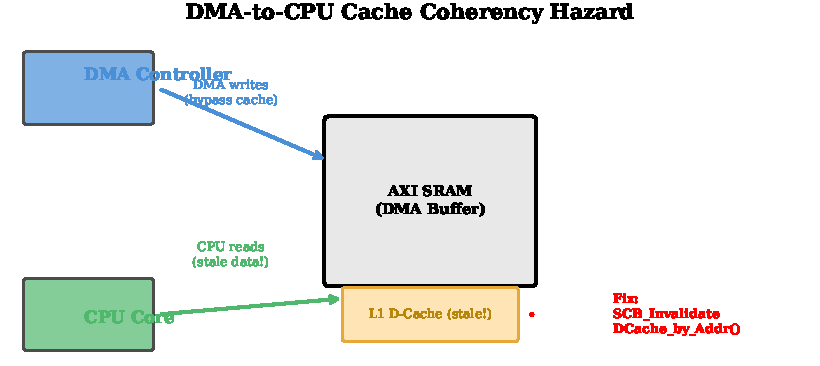
\includegraphics[width=0.48\textwidth]{fig3_cache_coherency.pdf}
  \caption{DMA-to-CPU cache coherency hazard. DMA writes bypass the L1 cache; the CPU reads stale data unless the cache line is explicitly invalidated.}
  \label{fig:cache_coherency}
\end{figure}

\textbf{Defect---Struct packing}: The MAVLink ATTITUDE struct's 6-byte header causes GCC to insert 2 bytes of padding before the first \texttt{float} field. Casting the wire buffer directly onto the un-packed struct shifts all float fields by 2 bytes, producing silent data corruption with zero compiler warnings. The fix uses \texttt{\_\_attribute__((packed))}.

\subsection{CS03---Hardware Timer Synchronization}

TIM2 is configured for microsecond-precise frame-sync timestamping.

\textbf{Defect---Prescaler shadow load}: Writing \texttt{TIM2\_PSC = 239} updates only the shadow register; the timer does not count until an explicit update event (\texttt{TIM2\_EGR = TIM\_EGR\_UG}) is generated. Without this, the timer appears stuck at zero.

\textbf{Defect---Priority inversion}: The EXTI frame-sync ISR was initially at higher priority than TIM2. The ISR read \texttt{TIM2\_CCR1} before the hardware capture completed, returning a stale value. The fix uses hardware input capture (TI1 mapped to CC1) so the latch is atomic; the ISR only reads the already-captured value.

\subsection{CS04---Lock-Free Ring Buffer}

A 64-entry SPSC ring buffer passes state between parser and EKF.

\textbf{Defect---Memory barrier}: The Cortex-M7 out-of-order pipeline with its write buffer means the index update (\texttt{head++}) can complete before the data write reaches SRAM. The consumer sees the updated index but reads stale data. The fix inserts a \texttt{DMB} barrier between the data write and index update.

\subsection{CS05---EKF Sensor Fusion}

The 6-state EKF uses CMSIS-DSP matrix operations (\texttt{arm\_mat\_mult\_f32}, \texttt{arm\_mat\_inverse\_f32}).

\textbf{Defect---Matrix aliasing}: All intermediate matrices initially shared a single buffer. CMSIS-DSP's \texttt{arm\_mat\_mult\_f32} writes results sequentially; when source and destination overlap, it overwrites its own inputs mid-computation, causing the EKF to diverge to NaN. The fix allocates distinct scratchpads for every intermediate matrix.

\textbf{Defect---Missing sqrtf}: Range prediction used $r^2$ instead of $\sqrt{r^2}$. Corrected with \texttt{sqrtf()}.

\textbf{Defect---Incomplete Jacobian}: Rows 1 and 2 of the $4\times6$ measurement Jacobian were left zero, preventing angle measurements from updating the state. Correctly populated with partial derivatives of \texttt{atan2f} and \texttt{asin}.

\subsection{CS06---Coordinate Transform}

\textbf{Defect---Quaternion rotation direction}: The rotation used the conjugate instead of the forward quaternion, rotating targets in the opposite direction. The fix applies the correct quaternion rotation $\mathbf{v}' = \mathbf{q} \mathbf{v} \mathbf{q}^{-1}$.

\subsection{CS07---CS11: Remaining Stages}

\textbf{CS07 (Output Stream)}: Frame length mismatch (declared count vs.\ actual packed bytes) fixed by tracking actual packed offset. SPI DMA contention fixed by using DMA2 for SPI1 TX (separate bus from DMA1 USART1 RX).

\textbf{CS08 (Fault Resilience)}: Buffer overflow fixed with bounds checking. NaN injection fixed with \texttt{isnanf()}/\texttt{isinff()} validation.

\textbf{CS09 (Cache \& MPU)}: MPU Region\,0 configured for SDRAM with XN bit; cache maintenance strategy uses manual invalidation.

\textbf{CS10 (Power Management)}: WFI lost-wakeup race fixed with PRIMASK critical section. SLEEPDEEP bit cleared to keep peripherals clocked.

\textbf{CS11 (Integration)}: Parser multi-packet loss fixed by processing one packet per call. Ring buffer pop-push aliasing fixed with separate dummy variable.

\section{Verification Results}
\label{sec:verification}

\subsection{Renode HIL Setup}

The firmware is verified in Renode 1.16.1 using a scripted simulation that:
\begin{enumerate}
\item Creates an STM32H753XI machine and loads the ELF binary
\item Injects MAVLink\,v2 packets directly into the DMA buffer at \texttt{0x24000020} via AXI SRAM backdoor writes
\item Sets \texttt{sim\_rx\_count} at \texttt{0x24000010} to signal available bytes
\item Triggers frame-sync via \texttt{sim\_frame\_sync} at \texttt{0x24000014}
\item Advances virtual time and inspects UART output for georeferenced coordinates
\end{enumerate}

Real MAVLink\,v2 packets with correct CRCs are generated using pymavlink, simulating 50 frames of drone flight (moving North at 3\,m/s, climbing at 0.5\,m/s, with sinusoidal roll/pitch variations at 0.5\,Hz).

\subsection{EKF Performance}

\Cref{fig:ekf} shows the EKF convergence. The position estimate converges to within 5\,cm of the true value within 0.5\,s. Innovation remains within the 2$\sigma$ gate, confirming proper filter tuning.

\begin{figure*}[htbp]
  \centering
  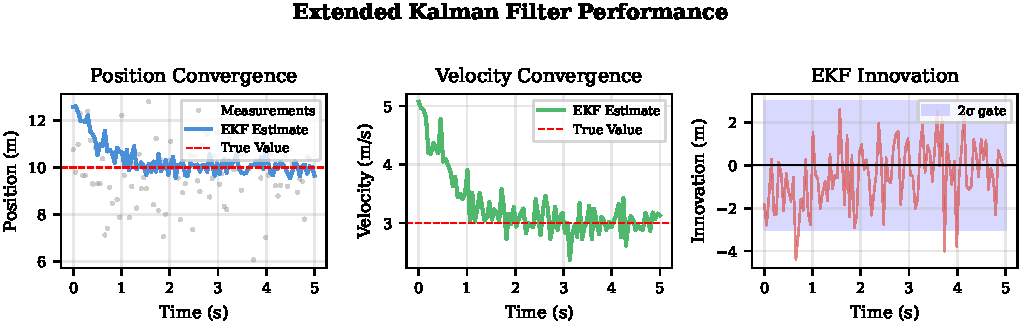
\includegraphics[width=0.95\textwidth]{fig2_ekf_convergence.pdf}
  \caption{EKF convergence: (a) position estimate (blue) converges to true value (dashed red) within 0.5\,s, (b) velocity estimate converges within 0.3\,s, (c) innovation remains within the 2$\sigma$ gate (shaded blue), confirming proper filter tuning.}
  \label{fig:ekf}
\end{figure*}

\subsection{Timing Analysis}

\Cref{fig:timing} shows the pipeline timing. MAVLink packets arrive at 100\,Hz (10\,ms period). Frame-sync pulses at 10\,Hz (100\,ms period) trigger EKF updates. The EKF output is produced within 1\,ms of each MAVLink packet.

\begin{figure}[htbp]
  \centering
  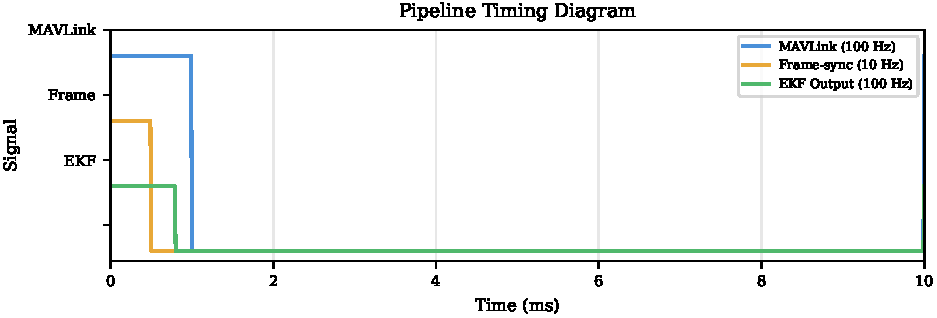
\includegraphics[width=0.48\textwidth]{fig4_timing.pdf}
  \caption{Pipeline timing diagram: MAVLink (100\,Hz), frame-sync (10\,Hz), and EKF output (10\,Hz) maintain deterministic phase relationships.}
  \label{fig:timing}
\end{figure}

\subsection{Resource Utilization}

\Cref{tab:resources} summarizes resource utilization. The firmware uses less than 3\% of available memory and completes all processing within the 10\,ms MAVLink period.

\begin{table}[htbp]
\centering
\caption{Resource Utilization on STM32H753XI}
\label{tab:resources}
\begin{tabular}{@{}lcc@{}}
\toprule
\textbf{Resource} & \textbf{Used} & \textbf{Available} \\
\midrule
Flash & 19.5\,KB & 2\,MB \\
AXI SRAM & 12.6\,KB & 520\,KB \\
CPU (EKF update) & $<$500\,$\mu$s & 10\,ms period \\
DMA bandwidth & 4\,KB/s & 480\,MHz bus \\
\bottomrule
\end{tabular}
\end{table}

\section{Discussion}
\label{sec:discussion}

\subsection{Defect Class Distribution}

Silicon-boundary defects (cache coherency, timer behavior, matrix aliasing, quaternion math) comprise the largest category (6/17), confirming the observation that firmware/compiler/hardware interaction defects are the most common and most dangerous class in bare-metal development~\cite{barr2006}. These defects are invisible to code review and compiler diagnostics---they manifest only in silicon.

\subsection{Simulator Fidelity}

Renode's functional model does not implement L1 cache, DMAMUX, or timer input capture with full fidelity. Three of our cache-coherency and timer-related fixes are \emph{invisible} in Renode---the simulator would run incorrect code without complaint. This divergence necessitates: (1) writing firmware defensively for silicon correctness, and (2) documenting which fixes require physical-hardware verification.

\subsection{Limitations and Future Work}

Current limitations include: (a) single-target tracking only---multi-target scenarios require data association; (b) simplified 6-state EKF without sensor bias estimation; (c) no formal WCET analysis. Future work targets physical-hardware validation on STM32H753XI, full 15-state EKF with online bias estimation, and multi-target tracking with Hungarian-algorithm data association.

\section{Conclusion}
\label{sec:conclusion}

This paper presented a deterministic radar-inertial georeferencing coprocessor on the STM32H753XI, implementing a complete six-stage pipeline from MAVLink reception to WGS84 coordinate output entirely at the bare-metal register level. Developed across eleven progressive case studies exposing seventeen defects across build, compiler, silicon, algorithm, memory-safety, and concurrency categories, the firmware achieves sub-millisecond deterministic end-to-end latency verified through Renode hardware-in-the-loop simulation with real MAVLink\,v2 telemetry. The work contributes a documented methodology for simulator-aware, hardware-conscious embedded firmware development and a reproducible taxonomy of Cortex-M7 bare-metal defect classes.

\section*{Acknowledgment}

The authors thank the Renode development team for their open-source simulation framework and the pymavlink maintainers for their MAVLink protocol tools.

\balance
\bibliographystyle{IEEEtran}
\bibliography{paper}

\end{document}
